\section{Background}
\label{sec:bg}

\paragraph{Setup and notation.}
We fix a decoder-only transformer of residual width $d$ and a layer index $\ell$, and write
$\boldsymbol{h}\in\mathbb{R}^{d}$ for the layer-$\ell$ residual-stream activation at the last token position.
Two populations of inputs are given, one exhibiting a desired behavior and one an undesired behavior, with
activation distributions $\pplus$ and $\pminus$ observed through i.i.d.\ samples
$\mathcal{D}^{+}=\{\boldsymbol{h}^{+}_{i}\}_{i=1}^{N_{+}}\sim\pplus$ and
$\mathcal{D}^{-}=\{\boldsymbol{h}^{-}_{j}\}_{j=1}^{N_{-}}\sim\pminus$, whose empirical measures we denote
$\pplushat$ and $\pminushat$. At inference, a steering map is applied to the layer-$\ell$ activation of each
decoded token, beginning with the last prompt token, and $\hquery$ denotes the activation currently being
steered. The map should move $\hquery$ toward regions of high density under $\pplus$ and low density under
$\pminus$, and it modifies no other activation. Vectors and vector fields are set in bold.

\paragraph{Spherical geometry of activations.}
Residual-stream norms concentrate tightly across inputs at a fixed layer, both
empirically~\citep{pham2024householder, you2026spherical} and as a consequence of the residual
architecture~\citep{yang2023spectral, xie2026controlled}. Figure~\ref{fig:norm-concentration} shows this
for the four models we study, for which the coefficient of variation of the layer-normalized last-token norm
lies between $2.5\%$ and $7.3\%$, and Appendix~\ref{appendix:norm_concentration} reports the same
measurement layer by layer and for four further architectures. We therefore model the state space as the
sphere $\Sph=\{\boldsymbol{x}\in\mathbb{R}^{d}:\lVert\boldsymbol{x}\rVert=R\}$ of radius $R$, the mean norm
over $\mathcal{D}^{+}\cup\mathcal{D}^{-}$, and restore the original norm of $\hquery$ after steering, so that
the intervention changes only the direction of the activation.

\begin{figure}[!ht]
\centering
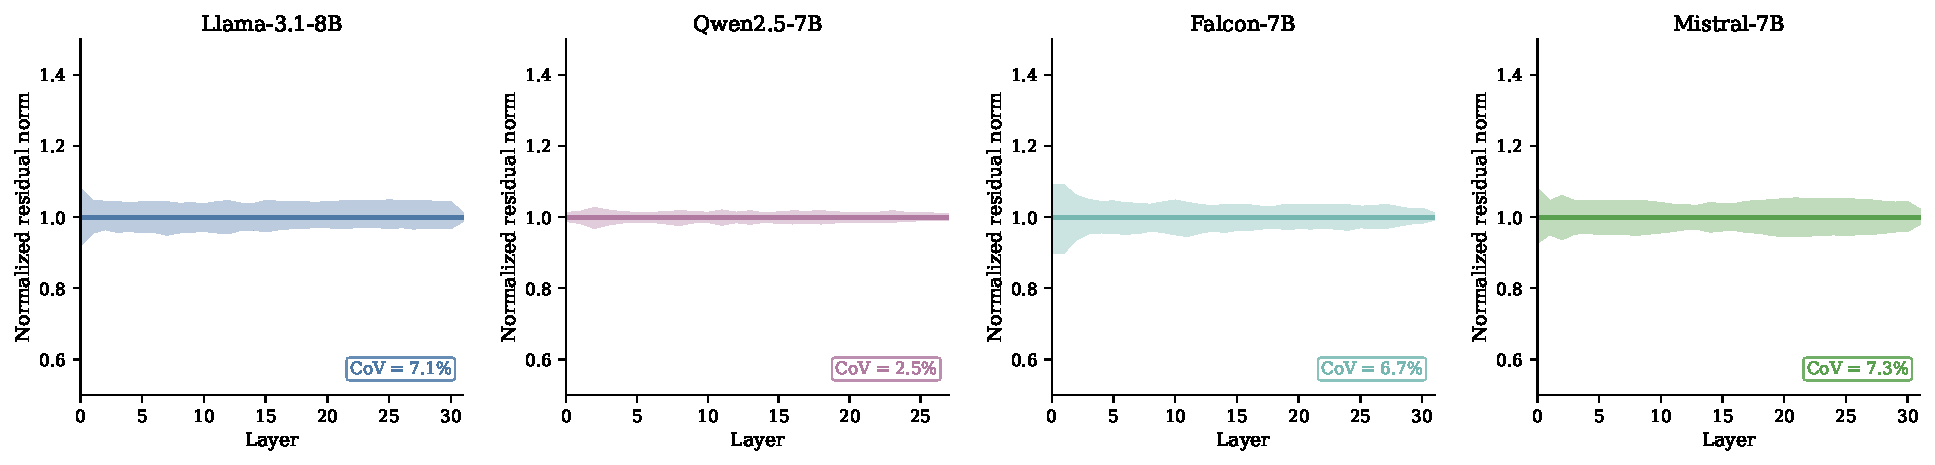
\includegraphics[width=\textwidth]{figures/norm_concentration.pdf}
\caption{Last-token residual-stream norms across layers on TruthfulQA for four LLMs, each divided by its
layer-wise mean. Dark and light bands show the 25th--75th percentiles. The coefficient of variation (CoV) is
reported per model.}
\label{fig:norm-concentration}
\end{figure}

\paragraph{Operations on $\Sph$.}
We write $\Pi_{\boldsymbol{x}}=\boldsymbol{I}-R^{-2}\boldsymbol{x}\boldsymbol{x}^{\top}$ for the projector
onto the tangent space at $\boldsymbol{x}$, $\nablaS f=\Pi_{\boldsymbol{x}}\nabla f$ for the Riemannian
gradient, and $d_{\Sph}(\boldsymbol{x},\boldsymbol{y})=R\arccos(R^{-2}\boldsymbol{x}^{\top}\boldsymbol{y})$
for the geodesic distance. The exponential map $\exp_{\boldsymbol{x}}(\boldsymbol{v})$ moves from
$\boldsymbol{x}$ along the tangent vector $\boldsymbol{v}$ for a geodesic arc of length
$\lVert\boldsymbol{v}\rVert$, and its inverse $\log_{\boldsymbol{x}}(\boldsymbol{y})$, defined for
$\boldsymbol{y}\neq-\boldsymbol{x}$, is the tangent vector at $\boldsymbol{x}$ that points toward
$\boldsymbol{y}$ with norm $d_{\Sph}(\boldsymbol{x},\boldsymbol{y})$:
\begin{equation}
\exp_{\boldsymbol{x}}(\boldsymbol{v})
= \cos\!\left(\frac{\lVert\boldsymbol{v}\rVert}{R}\right)\boldsymbol{x}
+ R\sin\!\left(\frac{\lVert\boldsymbol{v}\rVert}{R}\right)\frac{\boldsymbol{v}}{\lVert\boldsymbol{v}\rVert},
\qquad
\log_{\boldsymbol{x}}(\boldsymbol{y}) = \frac{\theta}{\sin\theta}\,\Pi_{\boldsymbol{x}}\boldsymbol{y},
\quad \theta = \frac{d_{\Sph}(\boldsymbol{x},\boldsymbol{y})}{R}.
\label{eq:expmap}
\end{equation}
The steering field derived below is a weighted sum of logarithm maps toward the contrastive samples, and
each steering step is an exponential map.

\section{LLM Steering as a Schr\"{o}dinger Bridge}
\label{sec:method}

Given contrastive activations $\mathcal{D}^{-}$ and $\mathcal{D}^{+}$, we need to decide both where to move
an activation and how strongly to intervene. \Cobras obtains the direction from a transport problem between
the undesired and desired populations on $\Sph$. It then adjusts the intervention using two signals: whether
the current token already lies on the desired side of the class boundary, and whether the prompt resembles
the data used to construct the intervention. Each update follows a geodesic and preserves the activation's
original norm.

The construction starts with a Schr\"{o}dinger bridge, which transforms one population into the other while
minimizing its departure from a reference diffusion (Section~\ref{subsec:sb}). We fit a transport plan to
contrastive samples and use it to weight the steering direction at the current activation
(Section~\ref{subsec:estimation}). Sections~\ref{subsec:strength} and~\ref{subsec:procedure} describe the
strength controls and the resulting inference procedure. Finally, Section~\ref{subsec:reduction} shows how
the density-ratio objective used by several existing methods arises as a limiting case.
Figure~\ref{fig:overview} summarizes the method.

\begin{figure}[!tb]
    \centering
    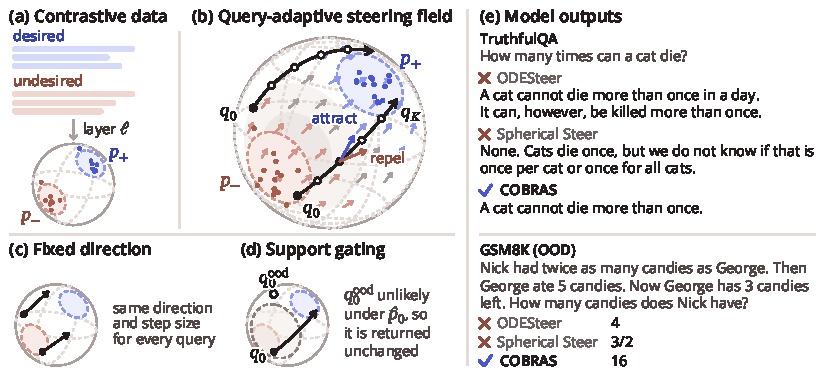
\includegraphics[width=0.8\linewidth]{figures/cobras_overview.pdf}
    \caption{Overview of \Cobras. \textbf{(a)} Contrastive activations at layer $\ell$ are projected onto
    $\Sph$. \textbf{(b)} Entropic optimal transport fits a coupling between the two populations. At each
    steering step, the coupling and the current activation determine weights for attraction toward desired
    samples and repulsion from undesired samples. \textbf{(c--d)} Whereas a fixed intervention treats every
    activation alike, \Cobras adjusts its direction and strength to the input; its support gate can leave
    unfamiliar prompts unchanged. \textbf{(e)} Example generations for TruthfulQA and an out-of-distribution
    GSM8K question, compared with ODESteer. The figure's iterates $q_k$ and support score $\hat p_0$
    correspond to $\boldsymbol{x}_k$ and $\hat p_{b_g}$ in the text.}
    \label{fig:overview}
\end{figure}

\subsection{From a population transport problem to a steering field}
\label{subsec:sb}

A direction that increases the likelihood of the desired behavior need not specify how to transform the
whole undesired population into the desired one. We begin with this population-level problem. A path measure
$P$ assigns probabilities to trajectories $(\boldsymbol{x}_t)_{t\in[0,1]}$ on $\Sph$; its marginal $P_t$
is the distribution of activations at time $t$. Taking Brownian motion on $\Sph$ as the reference $Q$, the
Schr\"{o}dinger bridge solves

\begin{equation}
P^{\star} = \operatorname*{arg\,min}_{P}\;\KL(P \,\Vert\, Q)
\qquad\text{s.t.}\qquad
P_{0} = \pminus, \quad P_{1} = \pplus ,
\label{eq:sb}
\end{equation}

Here $\KL$ is relative entropy between path measures, and $Q$ starts from the uniform distribution with
diffusivity $\sigma^2>0$. Thus the endpoint constraints specify the behavioral change, while the objective
selects the evolution that departs least from the reference motion. The time variable $t$ indexes this
transport between populations; it is separate from the token positions in a generated sequence.

The classical bridge solution is described by two positive functions, called Schr\"{o}dinger
potentials~\citep{leonard2013survey, chen2021likelihood, chen2023deep}. The potential
$\varphi(\boldsymbol{x},t)$ propagates information forward from the undesired population, and
$\psi(\boldsymbol{x},t)$ propagates information backward from the desired population. Both are functions
from $\Sph\times(0,1)$ to $(0,\infty)$, and $\nablaS$ differentiates their spatial argument with $t$
held fixed. We reserve these unhatted symbols for the continuous bridge; empirical kernel factors below
carry hats and explicit bandwidth subscripts. Their product gives the bridge's marginal density:

\begin{equation}
p_{t}(\boldsymbol{x})\;\propto\;\varphi(\boldsymbol{x},t)\,\psi(\boldsymbol{x},t),
\qquad
p_{0}(\boldsymbol{x})=\pminus(\boldsymbol{x}),\quad p_{1}(\boldsymbol{x})=\pplus(\boldsymbol{x}) .
\label{eq:product}
\end{equation}

Intuitively, $\varphi(\boldsymbol{x},t)$ describes how strongly the starting population reaches $\boldsymbol{x}$ at time
$t$, while $\psi(\boldsymbol{x},t)$ describes how strongly $\boldsymbol{x}$ connects to the target population in the
remaining time. The endpoint constraints determine the potentials, and the bridge adds the drift
$\sigma^2\nablaS\log\psi(\boldsymbol{x},t)$ to the reference diffusion.

To turn this stochastic evolution into a deterministic activation edit, we use its probability-flow ODE.
For the continuous bridge, this ODE has the same time marginals as the stochastic
process~\citep{song2020score}. Subtracting the diffusion contribution
$\tfrac{\sigma^2}{2}\nablaS\log p_t(\boldsymbol{x})$ from the bridge drift and using Eq.~\eqref{eq:product} gives
(Appendix~\ref{apx:static})

\begin{equation}
d\boldsymbol{x}_{t}
= \frac{\sigma^{2}}{2}\,\nablaS\log
  \frac{\psi(\boldsymbol{x}_{t},t)}{\varphi(\boldsymbol{x}_{t},t)}\,dt .
\label{eq:ldr}
\end{equation}

The two potentials therefore serve complementary purposes: their log-ratio supplies a direction toward
the desired population and away from the undesired one, while their product describes where the bridge
places probability mass. These identities motivate the direction and support score used below. Applying
them to finite samples and individual token activations requires the kernel construction and conditioning
choices in the next subsection.

\subsection{Computing the direction from contrastive samples}
\label{subsec:estimation}

\paragraph{Fit a transport plan offline.}
We first construct a coupling between the projected samples in $\mathcal{D}^{-}$ and $\mathcal{D}^{+}$.
The continuous bridge admits a static formulation over its endpoint coupling
(Appendix~\ref{apx:static}); we discretize that formulation using the empirical populations. To measure
proximity on $\Sph$, we use the geodesic kernel

\begin{equation}
K_{b}(\boldsymbol{x},\boldsymbol{y})
= \exp\!\left(-\frac{d_{\Sph}(\boldsymbol{x},\boldsymbol{y})^{2}}{2b}\right), \qquad b>0,
\label{eq:kernel}
\end{equation}

where $b$ has units of squared distance. Its form is motivated by the leading short-time behavior of the
Brownian transition density~\citep{de2022riemannian, chen2023logarithmic}. At our operating scale we use
$K_b$ as a chosen affinity kernel, rather than identifying it with the exact spherical heat kernel
(Remark~\ref{rem:prop1-tightness}).

Entropic optimal transport with this kernel yields the factorized plan

\begin{equation}
\pi^{\star}_{ji}=a^{-}_{j}\,a^{+}_{i}\,e^{-c_{ji}},
\qquad
c_{ji} = \frac{d_{\Sph}(\boldsymbol{h}^{-}_{j},\,\boldsymbol{h}^{+}_{i})^{2}}{2\varepsilon},
\label{eq:plan}
\end{equation}

The entry $\pi^\star_{ji}$ is the mass assigned from undesired sample $j$ to desired sample $i$.
The cost favors nearby pairs, and $\varepsilon=\sigma^2$ sets the entropic scale. The \emph{scalings}
$a^{-}_{j}>0$ and $a^{+}_{i}>0$ are scalar weights attached to samples.
We collect them in $\boldsymbol{a}^{-}=(a^{-}_{j})_{j=1}^{N_-}$ and
$\boldsymbol{a}^{+}=(a^{+}_{i})_{i=1}^{N_+}$. For the fixed data and entropic scale, these weights enforce
the empirical marginals: each row must sum to $1/N_-$ and each column to $1/N_+$.
We obtain them with alternating Sinkhorn updates~\citep{cuturi2013sinkhorn},

\begin{equation}
\log a^{-}_{j} = -\log N_{-} - \operatorname{logsumexp}_{i}\left[\log a^{+}_{i} - c_{ji}\right],
\qquad
\log a^{+}_{i} = -\log N_{+} - \operatorname{logsumexp}_{j}\left[\log a^{-}_{j} - c_{ji}\right].
\label{eq:sinkhorn}
\end{equation}

The resulting plan minimizes expected cost plus negative entropy over couplings with these marginals.
Its costs and scalings are computed once for a given contrastive dataset, model, and steering layer.

\paragraph{Evaluate the potentials at an activation.}
To obtain a steering direction at a token's current activation $\boldsymbol{x}\in\Sph$, we first extend
the fitted sample weights to empirical potential functions. Each sample contributes its kernel affinity
to $\boldsymbol{x}$, weighted by its Sinkhorn scaling, so the desired and undesired populations define

\begin{equation}
\widehat{\psi}_{b}(\boldsymbol{x}) = \sum\nolimits_{i=1}^{N_{+}}a^{+}_{i}\,K_{b}(\boldsymbol{x},\boldsymbol{h}^{+}_{i}),
\qquad
\widehat{\varphi}_{b}(\boldsymbol{x}) = \sum\nolimits_{j=1}^{N_{-}}a^{-}_{j}\,K_{b}(\boldsymbol{x},\boldsymbol{h}^{-}_{j}),
\label{eq:frozen-factors}
\end{equation}

where the evaluation bandwidth $b>0$ controls how broadly each population contributes around
$\boldsymbol{x}$, while $\varepsilon$ determines the transport plan fitted offline. In the continuous
bridge, the two potentials use bandwidths associated with elapsed and remaining transport time.
Because a decoded token has no prescribed bridge time, we use a common, fixed $b$ to construct a
stationary steering field; the continuous bridge's endpoint-matching guarantee applies to its
time-dependent evolution.

Following the log-ratio direction in Eq.~\eqref{eq:ldr}, we take the difference of the two empirical
potentials' log-gradients. For the geodesic kernel, the identity
$\nablaS d_{\Sph}(\boldsymbol{x},\boldsymbol{h})^2=-2\log_{\boldsymbol{x}}(\boldsymbol{h})$ expresses
each log-gradient as a weighted average of tangent vectors toward the samples. For the desired population,
this gives

\begin{equation}
\nablaS\log\widehat{\psi}_{b}(\boldsymbol{x})
= \frac{1}{b}\sum_{i=1}^{N_{+}} w^{+}_{i}(\boldsymbol{x})\,\log_{\boldsymbol{x}}(\boldsymbol{h}^{+}_{i}),
\qquad
w^{+}_{i}(\boldsymbol{x})
= \mathrm{softmax}_{i}\!\left[\log a^{+}_{i}
   - \frac{d_{\Sph}(\boldsymbol{x},\boldsymbol{h}^{+}_{i})^{2}}{2b}\right],
\label{eq:grad-psi}
\end{equation}

with the corresponding expression for $\nablaS\log\widehat{\varphi}_{b}(\boldsymbol{x})$ obtained by
summing over $\mathcal{D}^{-}$ (Appendix~\ref{app:grad-psi}); both identities hold away from the samples'
antipodes. The normalized weight $w_i^{+}(\boldsymbol{x})$ combines the desired sample's proximity to
$\boldsymbol{x}$ with its fitted scaling $a_i^{+}$. Subtracting the undesired log-gradient therefore
combines attraction toward desired samples with repulsion from undesired samples, providing the
weighted log-map construction that we refine below.

\paragraph{Condition the weights on the current activation.}
The weights in Eq.~\eqref{eq:grad-psi} use the transport plan through a single fitted scaling for each
sample. To make the direction depend on which samples the plan connects near $\boldsymbol{x}$,
\Cobras replaces these scalings with conditional multipliers. For a desired sample $i$, we aggregate
its connections to undesired samples, weighting each connection by the undesired sample's proximity
to $\boldsymbol{x}$. Applying the same construction from desired samples to an undesired sample $j$
gives the two positive multiplier functions

\begin{align}
\log m^{+}_{i,b}(\boldsymbol{x})
&= \operatorname{logsumexp}_{j}\!\left[
   \log a^{-}_{j}
   - \frac{d_{\Sph}(\boldsymbol{x},\boldsymbol{h}^{-}_{j})^{2}}{2b}
   - c_{ji}\right],
\label{eq:ext-psi}\\[2pt]
\log m^{-}_{j,b}(\boldsymbol{x})
&= \operatorname{logsumexp}_{i}\!\left[
   \log a^{+}_{i}
   - \frac{d_{\Sph}(\boldsymbol{x},\boldsymbol{h}^{+}_{i})^{2}}{2b}
   - c_{ji}\right].
\label{eq:ext-phi}
\end{align}

In the first expression, the kernel centered at $\boldsymbol{x}$ emphasizes nearby undesired samples,
and the pairwise cost $c_{ji}$ determines how strongly each sample in that neighborhood contributes to
desired sample $i$. The relation
$a^{+}_{i}m^{+}_{i,b}(\boldsymbol{x})=\sum_j\pi^\star_{ji}K_b(\boldsymbol{x},\boldsymbol{h}^{-}_j)$
identifies $m^{+}_{i,b}(\boldsymbol{x})$ as the kernel-weighted transport mass arriving at desired sample $i$,
divided by its scaling $a_i^{+}$. We then combine the multiplier with the desired sample's own
proximity to $\boldsymbol{x}$ and normalize across desired samples. The resulting weights and
steering field are

\begin{align}
\bar{w}^{+}_{i}(\boldsymbol{x})
&= \mathrm{softmax}_{i}\!\left[
  \log m^{+}_{i,b}(\boldsymbol{x})
  - \frac{d_{\Sph}(\boldsymbol{x},\boldsymbol{h}^{+}_{i})^{2}}{2b}\right],
\label{eq:weights-pos}\\[2pt]
\boldsymbol{v}(\boldsymbol{x})
&= \sum\nolimits_{i=1}^{N_{+}} \bar{w}^{+}_{i}(\boldsymbol{x})\,\log_{\boldsymbol{x}}(\boldsymbol{h}^{+}_{i})
- \sum\nolimits_{j=1}^{N_{-}} \bar{w}^{-}_{j}(\boldsymbol{x})\,\log_{\boldsymbol{x}}(\boldsymbol{h}^{-}_{j}),
\label{eq:cobras-field}
\end{align}

where $\bar w_j^{-}(\boldsymbol{x})$ is obtained by replacing $m^{+}_{i,b}(\boldsymbol{x})$ and
$\boldsymbol{h}_i^{+}$ with $m^{-}_{j,b}(\boldsymbol{x})$ and $\boldsymbol{h}_j^{-}$ and normalizing
over undesired samples. Thus attraction and repulsion each depend on proximity within one population
and transport connections to the other population near $\boldsymbol{x}$. Since the integrator
normalizes $\boldsymbol{v}(\boldsymbol{x})$ before stepping, we omit the common prefactors $1/b$ and
$\sigma^2/2$.

At each steering iterate, we recompute the conditional multipliers at the updated activation and
use them as fixed coefficients in the weighted log-map construction. This defines the field in
Eq.~\eqref{eq:cobras-field}; differentiating through the multipliers would introduce additional terms
derived in Appendix~\ref{apx:omitted-term}. The common bandwidth $b$ makes this construction and its
density-ratio limit explicit, while the implementation selects bandwidths separately for each activation
and population. Appendix~\ref{app:grad-psi} describes this adaptive choice and compares it with the
fixed-bandwidth version.

\subsection{Controlling when and how much to steer}
\label{subsec:strength}

We follow the normalized direction $\boldsymbol{v}/\lVert\boldsymbol{v}\rVert$, so its magnitude cannot
reduce the intervention on a token that already exhibits the desired behavior or on an unfamiliar prompt.
We handle these cases with two factors in $[0,1]$: a per-token side factor $s$ and a per-prompt support gate
$g$. Their product scales the user-selected steering strength $T$.

\paragraph{Side factor: reduce steering on the desired side.}
We estimate which side of the behavioral boundary the current token occupies using a simple auxiliary
class model. Let $\bar{\boldsymbol{h}}^{\pm}$ be the means of the projected contrastive samples. Model
the classes by von Mises--Fisher distributions with opposite mean directions $\pm\boldsymbol{\mu}$,
equal prior probabilities, and shared concentration $\kappa$. The class axis and posterior probability of
the undesired class are

\begin{align}
\boldsymbol{\mu}
&= \frac{\bar{\boldsymbol{h}}^{+}-\bar{\boldsymbol{h}}^{-}}
       {\lVert\bar{\boldsymbol{h}}^{+}-\bar{\boldsymbol{h}}^{-}\rVert},
\label{eq:mu}\\[2pt]
s(\boldsymbol{x}) &= \bigl(1+e^{\,2\kappa\langle\boldsymbol{x}/R,\,\boldsymbol{\mu}\rangle}\bigr)^{-1}.
\label{eq:side}
\end{align}

The shared normalizing constants cancel, giving log-odds
$2\kappa\langle\boldsymbol{x}/R,\boldsymbol{\mu}\rangle$ in favor of the desired class
(Appendix~\ref{apx:ldr-formalize}). Consequently, $s$ is larger on the undesired side, equals $1/2$ at the
boundary, and decreases smoothly on the desired side. It attenuates steering rather than imposing a hard
stop at the boundary. We evaluate $s$ on each token's incoming activation and hold it fixed during that
token's integration steps.

\paragraph{Support gate: reduce steering on unfamiliar prompts.}
A class posterior alone cannot determine whether the fitted intervention is appropriate for a prompt.
For example, a truthfulness intervention may alter a math problem whose activations lie far from the
contrastive samples. A ratio can remain large even when both of its factors are small. Their product
retains this information, motivating a support score based on Eq.~\eqref{eq:product}. Using the fixed
Sinkhorn scalings and a gate bandwidth $b_g$, we define

\begin{equation}
\begin{aligned}
u(\boldsymbol{x}) &= -\log\hat p_{b_{g}}(\boldsymbol{x}), \\
\log\hat p_{b_{g}}(\boldsymbol{x})
&= \operatorname{logsumexp}_{j}\!\left[\log a^{-}_{j}
  -\frac{d_{\Sph}(\boldsymbol{x},\boldsymbol{h}^{-}_{j})^{2}}{2b_{g}}\right] \\
&\quad + \operatorname{logsumexp}_{i}\!\left[\log a^{+}_{i}
  -\frac{d_{\Sph}(\boldsymbol{x},\boldsymbol{h}^{+}_{i})^{2}}{2b_{g}}\right],
\end{aligned}
\label{eq:support-score}
\end{equation}

Here $\hat p_{b_g}(\boldsymbol{x})=\widehat{\varphi}_{b_g}(\boldsymbol{x})\widehat{\psi}_{b_g}(\boldsymbol{x})$ is an unnormalized support score built from the kernel
factors; large $u$ indicates low support. At this chosen bandwidth it serves as a proxy for the bridge
marginal, rather than an exact time marginal of the continuous bridge. As $b_g\to0$, $2b_gu(\boldsymbol{x})$
approaches the sum of squared distances to the nearest sample in each population
(Lemma~\ref{lem:gate-nn}). The score thus connects the potential product to a local measure of proximity
to the contrastive data.

To interpret this score on the inputs encountered at inference, we calibrate it on in-distribution
\emph{prompt} activations $\mathcal{D}_{\mathrm{ref}}$, held out from evaluation. Each reference activation
is taken at layer $\ell$ and the last prompt position, and projected onto $\Sph$ before scoring. We rank a
query's score against these reference scores and convert its rank to a gate:

\begin{equation}
r(\boldsymbol{x})
= \frac{\bigl|\{\boldsymbol{z}\in\mathcal{D}_{\mathrm{ref}} : u(\boldsymbol{z}) < u(\boldsymbol{x})\}\bigr|}
       {|\mathcal{D}_{\mathrm{ref}}|},
\qquad
g(\boldsymbol{x}) = \mathrm{clamp}\!\left(\frac{1-r(\boldsymbol{x})}{1-p},\,0,\,1\right),
\label{eq:gate}
\end{equation}

The coverage parameter $p\in(0,1)$ sets the rank below which the gate is one. Above that rank the gate
decreases linearly, reaching zero when the query score exceeds all reference scores. We compute
$g_q$ once on the last prompt token and hold it fixed throughout generation, so a prompt with $g_q=0$
receives no steering. The ungated configuration sets $g_q=1$ directly.

Calibration on prompts matches the layer and token position where the gate is used, rather than assuming
that contrastive question--answer activations have the same score distribution. It requires no OOD data.
Under the continuous in-distribution percentile model, a fraction $p$ of prompts receives full strength
and $\mathbb{E}[g]=(1+p)/2$; a finite reference set introduces rank discretization
(Appendix~\ref{apx:ood-gate}). These are calibration properties, while separation of unfamiliar prompts
depends on their scores. The appendix reports the measured in-distribution coverage and OOD separation.

\subsection{Applying the intervention during generation}
\label{subsec:procedure}

The direction and strength controls now define the activation edit. For the incoming activation
$\hquery$, set $\boldsymbol{x}_0=R\hquery/\lVert\hquery\rVert$, evaluate $s(\boldsymbol{x}_0)$, and use
the prompt's cached gate $g_q$. With $K$ geodesic Euler steps, the update is

\begin{equation}
\Delta = \frac{\pi}{2}\,T\,s(\boldsymbol{x}_{0})\,g_{q}\,\frac{R}{K},
\qquad
\boldsymbol{x}_{k+1}
= \exp_{\boldsymbol{x}_{k}}\!\left(\Delta\,
  \frac{\boldsymbol{v}(\boldsymbol{x}_{k})}{\lVert\boldsymbol{v}(\boldsymbol{x}_{k})\rVert}\right),
\label{eq:step}
\end{equation}

Each nonzero step traverses an arc of length $\Delta$. At full strength ($s=g_q=1$), the total path length
is $\tfrac{\pi}{2}TR$, so $T$ expresses the steering budget in units of a quarter great circle.
We recompute the conditional multipliers and direction at every iterate, while keeping $s$ and $g_q$
fixed during these $K$ steps. After integration, the activation returned to the model is
$\lVert\hquery\rVert\boldsymbol{x}_K/R$, which restores its original norm. If the step length or field
is zero, the corresponding update is zero.

\paragraph{Offline preparation and online cost.}
For each contrastive dataset, model, and layer, preparation projects the samples onto $\Sph$, sets the
transport scale from their spacing, fits the Sinkhorn scalings, and computes the class axis and reference
support scores. During generation, the intervention runs on the last-token activation at each decoding
step, starting with the last prompt token. No model weights change. For the dense construction shown
here, each field evaluation uses $O(N_-N_+)$ work to form the conditional multipliers and
$O(d(N_-+N_+))$ work for distances and weighted tangent vectors; the transport cost matrix is stored
offline. Each steered token requires $K$ such evaluations.
Algorithm~\ref{alg:cobras} gives the pseudocode, and
Appendix~\ref{appendix:implementation_details} lists the experimental settings.

The bridge supplies the log-ratio form of the direction and the product form of the support score.
\Cobras turns those identities into a practical intervention through the geodesic kernel, conditional
weights, normalized steps, and strength controls. Its endpoint transport objective motivates these
operations; exact population transport is not a guarantee of the resulting token-level procedure.

\subsection{Connection to density-ratio steering}
\label{subsec:reduction}

We now relate the construction to a familiar steering objective. Several methods can be expressed as
following a log-density-ratio gradient~\citep{rimsky2024steering, zhaoodesteer, li2023inference},

\begin{equation}
  \boldsymbol{v}(\boldsymbol{x}) \;\propto\; \nabla \log \frac{\pplus(\boldsymbol{x})}{\pminus(\boldsymbol{x})},
  \label{eq:ldr-ideal}
\end{equation}

which combines attraction toward regions favored by $\pplus$ with repulsion from regions favored by
$\pminus$. For isotropic Gaussians $\mathcal{N}(\boldsymbol{\mu}_{\pm},\boldsymbol{I}_d)$, this gradient
is the constant vector $\boldsymbol{\mu}_+-\boldsymbol{\mu}_-$ used by Contrastive Activation Addition
(CAA)~\citep{rimsky2024steering}. Appendix~\ref{apx:ldr-formalize} and
Table~\ref{tab:steering_framework} describe the corresponding parameterizations for other methods.

The bridge provides a population transport objective from which a log-ratio field follows. For the
sample-based construction, the ordinary kernel density-ratio field is recovered when transport costs
become negligible. Define

\begin{equation}
\hat p^{\pm}_{b}(\boldsymbol{x})
= \frac{1}{N_{\pm}}\sum\nolimits_{k=1}^{N_{\pm}} K_{b}(\boldsymbol{x},\boldsymbol{h}^{\pm}_{k}),
\qquad
\boldsymbol{v}^{\mathrm{kde}}_{b}(\boldsymbol{x})
= b\,\nablaS\log\frac{\hat p^{+}_{b}(\boldsymbol{x})}{\hat p^{-}_{b}(\boldsymbol{x})}
\label{eq:ldr-kde}
\end{equation}

where the kernel's common normalizing constant cancels in the ratio. By Eq.~\eqref{eq:grad-psi}, this
field uses uniform multipliers within each population. As $\varepsilon$ grows, the costs $c_{ji}$ tend
to zero, the reference weights $K_{\varepsilon}(\boldsymbol{h}^{-}_{j},\boldsymbol{h}^{+}_{i})$ become uniform, and the optimal coupling approaches the
independent plan $\pi^\star_{ji}=1/(N_-N_+)$. The following proposition quantifies how the conditional
field approaches the kernel density-ratio field in this regime.

\begin{proposition}[Reduction to the kernel density-ratio drift]
\label{prop:ldr-limit}
Fix $\mathcal{D}^{\pm}\subset\Sph$, an entropic scale $\varepsilon>0$ and an evaluation bandwidth $b>0$, put
$c_{\max}=\max_{j,i}c_{ji}$, and let $(\boldsymbol{a}^{-},\boldsymbol{a}^{+})$ be an iterate obtained after a complete
Sinkhorn sweep of Eq.~\eqref{eq:sinkhorn}, or its fixed point. Then at every $\boldsymbol{x}\in\Sph$ not antipodal to
a sample, the field of Eq.~\eqref{eq:cobras-field} satisfies
\begin{equation}
\bigl\lVert\,\boldsymbol{v}(\boldsymbol{x})-\boldsymbol{v}^{\mathrm{kde}}_{b}(\boldsymbol{x})\,\bigr\rVert
\;\le\; 2\pi R\,\bigl(e^{c_{\max}}-1\bigr).
\label{eq:prop1-bound}
\end{equation}
Since $c_{\max}\le\pi^{2}R^{2}/(2\varepsilon)$, holding $\mathcal{D}^{\pm}$ and $b$ fixed and letting
$\varepsilon\to\infty$ drives the right-hand side to zero, so $\boldsymbol{v}$ converges to
$\boldsymbol{v}^{\mathrm{kde}}_{b}$ uniformly over points that are not antipodal to a sample.
\end{proposition}

The limit holds at a fixed evaluation bandwidth $b$: it removes the information carried by the coupling
while retaining a nondegenerate kernel density-ratio field. At finite $\varepsilon$, the transport
weights modify that field using relationships between the two populations. The bound gives an asymptotic
$O(1/\varepsilon)$ rate; it is not tight at our operating scale
(Remark~\ref{rem:prop1-tightness}). The proof is in Appendix~\ref{apx:proof-ldr-limit}.

A separate statistical question is whether the kernel estimates recover the population objective in
Eq.~\eqref{eq:ldr-ideal}. Under the smoothness and sampling conditions of Remark~\ref{rem:consistency},
shrinking $b$ with sample size gives consistency of the unscaled log-density-ratio gradient wherever both
population densities are bounded away from zero. That sampling limit differs from the fixed-$b$ transport
limit above and does not provide a combined guarantee for the deployed steering procedure.
